%! TEX program = xelatex
%
% Compile with xelatex
%
\documentclass[a4paper,12pt]{book}

% Packages

%
\usepackage{fontspec}
\usepackage[english, greek]{babel} % Η τελευταία γλώσσα είναι η βασική (Ελληνικά)

% Fonts
\setmainfont{Liberation Serif}
%\setmainfont{Times New Roman}
%\setmonofont{Courier New}
%\setmonofont{Fira Code}

% Math
\usepackage{amsmath, amssymb, amsfonts}
\usepackage{siunitx}

% Figures
\usepackage{graphicx}
\usepackage{float} % For [H] flag
\graphicspath{{./figures/}} % path for figures

% Colors
\usepackage{xcolor}

% hyperref
\usepackage{hyperref}
\hypersetup{
    colorlinks=false,
    linktocpage=true,
    linkbordercolor=blue,
    filebordercolor=magenta,
    urlbordercolor=cyan,
}

% title page
\usepackage{titling}

%


\begin{document}

\frontmatter

% Σελίδα εξωφύλλου
% Title Page for NT collaborative book
%
\begin{titlingpage}
\begin{center}
%
\vspace*{6mm}
\begin{minipage}{0.1\textwidth}
    \quad
\end{minipage}
\begin{minipage}{0.19\textwidth}
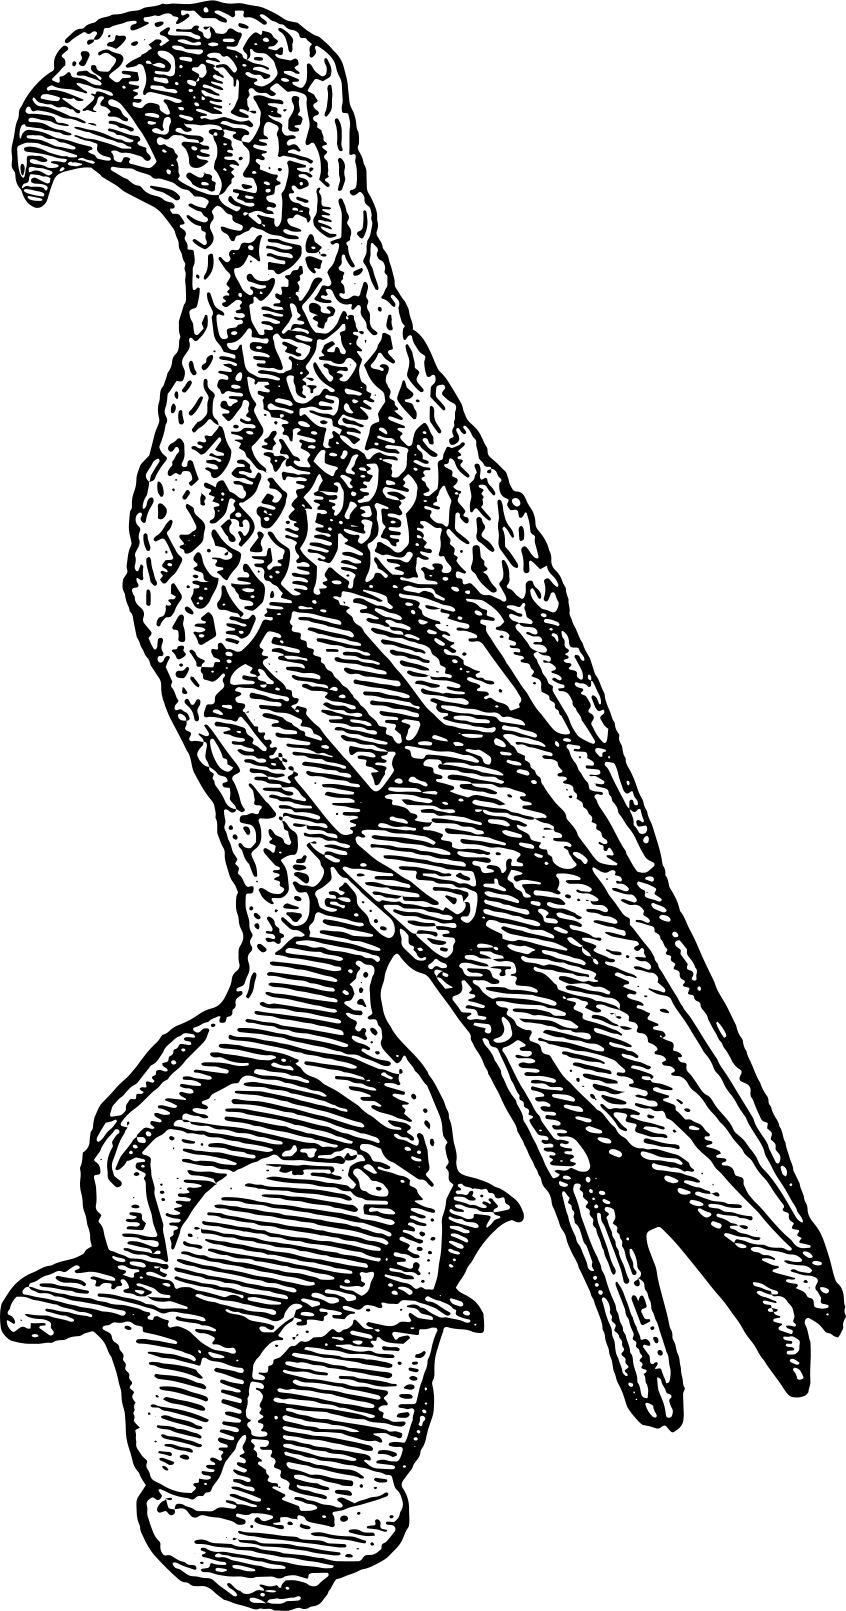
\includegraphics[width=0.35\linewidth]{uoi-logo.png}
\end{minipage}
\begin{minipage}{0.38\textwidth}
\begin{center}
{\normalfont\normalsize\scshape Πανεπιστήμιο Ιωαννίνων}\\[0.7mm]
{\normalfont\normalsize\scshape Σχολή Θετικών Επιστημών}\\[0.7mm]
{\normalfont\normalsize\scshape Τμήμα Φυσικής}\\[0.7mm]
\end{center}
\end{minipage}
\begin{minipage}{0.1\textwidth}
    \quad
\end{minipage}
\begin{minipage}{0.19\textwidth}
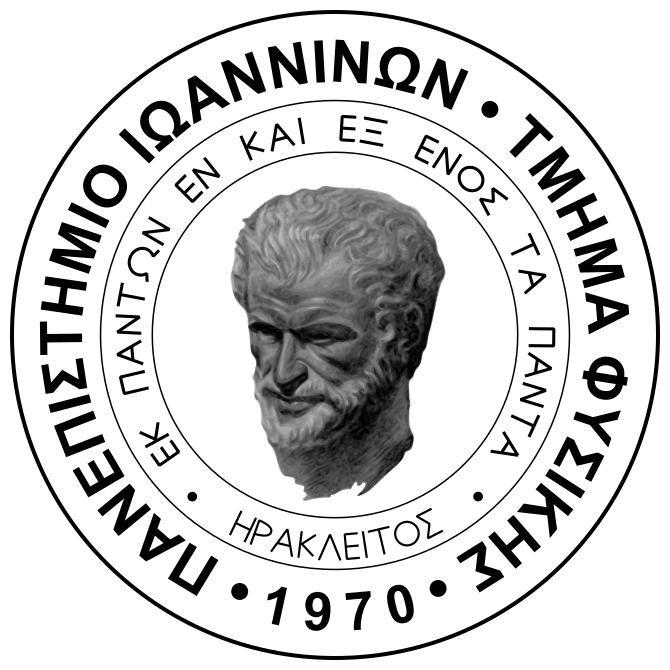
\includegraphics[width=0.75\linewidth]{physics-uoi-logo.png}
\end{minipage}
%
\\ \vspace*{20mm}
%
\rule[0.5ex]{\linewidth}{2pt}\vspace*{-\baselineskip}\vspace*{2.5pt}
\rule[0.5ex]{\linewidth}{1pt}\\[2mm]
{\normalfont\LARGE Φυσική Γενικού Λυκείου}\\[4mm]
{\normalfont\large Μία σύνοψη}\\[1mm]
\rule[0.5ex]{\linewidth}{1pt}\vspace*{-\baselineskip}\vspace{3.5pt}
\rule[0.5ex]{\linewidth}{2pt}\\
\vspace{12mm}
{\normalfont\itshape Ένα συνεργατικό βιβλίο γραμμένο από}\\[2mm]
{\normalfont\large Φοιτητές και Φοιτήτριες του Π.Ι.}\\
\vspace{5mm}
{\normalfont\itshape Στο πλαίσιο του μαθήματος}\\[1mm]
{\normalfont\large Νέες Τεχνολογίες στη Διδακτική των Φυσικών Επιστημών}\\
\vspace{10mm}
{\normalfont\large Επιβλέπων/Συντονιστής: Λάμπρος Τριφύλλης}\\
\vfill
{\large Ιωάννινα, 2026}
\end{center}
\end{titlingpage}


% Πρόλογος
\chapter*{Περίληψη}
\addcontentsline{toc}{chapter}{Περίληψη}

Το παρόν project αποτελεί μια διαδραστική εκπαιδευτική προσομοίωση στο πλαίσιο του προπτυχιακού
μαθήματος ``Νέες Τεχνολογίες στη Διδακτική των ΦΕ'' του Τμήματος Φυσικής του Πανεπιστημίου
Ιωαννίνων. Κύριος στόχος είναι η εξοικείωση των φοιτητών/τριών με τις σύγχρονες συνεργατικές
μεθόδους που χρησιμοποιούνται στην επιστημονική έρευνα και την ανάπτυξη λογισμικού. Μέσα από τη
συνδυαστική χρήση του \LaTeX{} για την επιστημονική συγγραφή, της \texttt{Python (Matplotlib)} για
την προγραμματιστική παραγωγή γραφημάτων, και του \texttt{Git/GitHub} για τον έλεγχο εκδόσεων
(version control) και τη διαχείριση κλάδων (branch management), οι συμμετέχοντες συνεργάζονται
δυναμικά για τη σύνταξη ενός ενιαίου επιστημονικού συγγράμματος Φυσικής.


% Περιεχόμενα
\tableofcontents

\mainmatter

% Student chapters
% Note: please insert a new line below, with the name of the tex file containing your chapter.
% For example: \input{chapters/ph01234}

\end{document}
